%\setcounter{page}{1}
\setcounter{equation}{0}
\setcounter{figure}{0}

\section{Weighing an Electron}

Name \rule{2.0in}{0.1pt}\hfill{}Section \rule{1.0in}{0.1pt}\hfill{}Date
\rule{1.0in}{0.1pt}

\textbf{Objective}

To investigate the force on a charged particle due to a magnetic field and 
learn how the motion of the particle can be used to weigh it.

\textbf{Apparatus}

\begin{itemize}

\item $e/m$ apparatus

\item Low- and high-voltage power supplies

\item Analog ammeter and digital multi-meter

\item Flashlight

\end{itemize}

\textbf{Overview}

Mass spectroscopy is an experimental technique that is used to determine
the mass of atoms, molecules, and sub-atomic particles.
The central idea is to make a version of the particle carrying an electric
charge ({\it e.g.}, a bare electron, an ionized molecule, {\it etc}), accelerate it
through an electric potential, and then inject it into a magnetic field.
If properly oriented, the magnetic field will bend the object into
a curved path.
The amount of curvature depends on the mass of the object and the electric
charge it is carrying so that different mass particles with the same charge will
bend by different amounts.
Measuring this bend is equivalent to a mass measurement.
This method is widely used to do things like determine the mass of newly discovered particles,
hunt for oil, and even validate the authenticity of works of art.

\textbf{Activity 1: Magnetic Force on a Charged Particle}

It has been found by careful measurements that the force $\vec F_B$ on a charged
particle due to a magnetic field is
\begin{equation}
\vec F_B = q \vec v \times \vec B
\end{equation}
where $q$ is the electric charge of the particle, $\vec v$ is its velocity,
and $\vec B$ is the local magnetic field.
Find the relevant sections in your text for a discussion of the cross product.

(a) The figure below shows the relationship between $\vec F_B$, $\vec v$,
and $\vec B$.
How is the magnitude of the cross product $\vec v \times \vec B$ related to
the magnitude of $v$, $B$, and $\theta$ the angle between $\vec v$ 
and $\vec B$?
\vspace{5mm}

\begin{figure}[h!]
\begin{center}
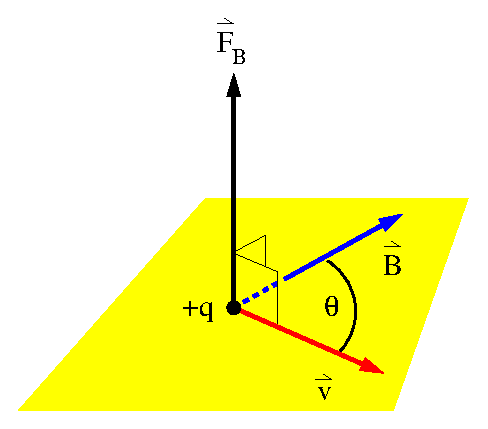
\includegraphics[height=2.0in]{eoverm/vCrossB.eps}
\caption{Vectors associated with the magnetic force. \hfill}
\end{center}
\end{figure}

(b) Consider a situation where the magnetic field is uniform in space
and points in the $z$ direction $\vec B = B \hat k$ and the velocity of
the charged particle is in the $y$ direction $\vec v = v \hat j$. 
What is $\theta$, the angle between the magnetic field and velocity vectors?
What is 
$\vec F_B$ in terms of the magnitudes of $q$, $v$, and $B$ and the appropriate unit
vectors?
\vspace{25mm}

%\newpage

(c) Describe the trajectory of the charged particle.
What is the $z$ component of its trajectory?
\vspace{30mm}

(d) What is the magnitude of the magnetic force as this charged particle
moves through the region of the magnetic field?
Does this magnitude change as the particle moves through the field?
\vspace{15mm}

(e) How are the directions of $\vec F_B$ and $\vec v$ related?
\vspace{15mm}


\textbf{Activity 2: Relating $\vec F_B$ to the Kinematics}

At the end of the previous section you should have found that the magnitude 
of the magnetic force is $|qvB|$ and that $\vec v$ and $\vec B$ are
always perpendicular to one another.

(a) What type of force have we encountered 
that is perpendicular to the velocity and constant in magnitude?
(Hint: Recall some of the applications of Newton's Laws in your text.)
\vspace{15mm}

(b) How is centripetal acceleration related to $v$ and $r$ (the radius of the
circular motion)? From Newton's 2nd Law, what is the expression for the magnitude of the centripetal force $|\vec F_c|$?
\vspace{15mm}

\newpage

(c) If the magnetic force from Activity 1 is the only force acting on a particle and we know it moves in a circle, then this force must be the centripetal force causing it to move in a circle.  Equate the expressions for the magnitudes of $\vec F_B$ (from 1(d)) and $\vec F_c$ (from 2(b)). 
Solve for the mass $m$ in terms of the radius $r$ of the particle's path,
$|q|$, $v$, and $B$.
\vspace{35mm}


(d) Using your result from 2(c), answer the following questions.
For two particles with the same charge and velocity, but different mass, which one will have the larger path radius?
How will increasing the velocity change the path radius?
\vspace{30mm}

(e) Remember that in a mass spectrometer, the particle is first accelerated
across an electric potential difference.
Typically, we know the kinetic energy $K$ of the charged particle after this
acceleration instead of the velocity.
Rewrite your result in 2(c) in terms of the kinetic energy $K$ instead of the
velocity $v$.
\vspace{30mm}

(f) The electron `falls' across a potential difference created by the accelerating voltage
to gain a velocity $v$ before it enters the magnetic field region.
Assuming the electron starts from rest, what is the relationship between the accelerating
voltage and the kinetic energy $K$ when it leaves the accelerating region and
enters the magnetic field? 
Combine this result with the one from part 2(e) to get an expression for 
the mass of the electron in terms of the accelerating voltage $V$, the
electron charge $e$, the radius of the electron's path $r$, and 
the magnetic field $B$.
\vspace{30mm}

%(f) We will use the mass spectrometer to measure the radius of the particle's trajectory
%and then derive a mass from that measurement. Rearrange your result from
%section 2.e to isolate the mass $m$ on one side of the equation.
%\vspace{30mm}

\textbf{Activity 3: Predictions for a Charged Particle in a Magnetic Field}

We now have the mathematical tools to understand the motion of a charged
particle in a magnetic field so we can start  investigating the physics.

(a) First make some predictions.
If $\vec B = B \hat k$ and $\vec v = v \hat j$, then what direction is
$\vec v \times \vec B$?
\vspace{15mm}

\newpage

(b) What direction is $\vec F_B$ for a positively charge particle 
if $\vec B = B \hat k$ and $\vec v = v \hat j$?
\vspace{15mm}

(c) What direction is $\vec F_B$ for a negatively charge particle
if $\vec B = B \hat k$ and $\vec v = v \hat j$?
\vspace{15mm}

\textbf{Activity 4: Measuring a Charged Particle in a Magnetic Field}

The last piece of the puzzle before we start measuring things is the magnetic field
$\vec B$.
The apparatus you are using consists of a pair of wire coils (called Helmholtz coils) and
an electron gun that produces a beam of electrons.
See Figure 2 and identify the Helmholtz coils on your apparatus.
\begin{figure}[hbt]
\begin{center}

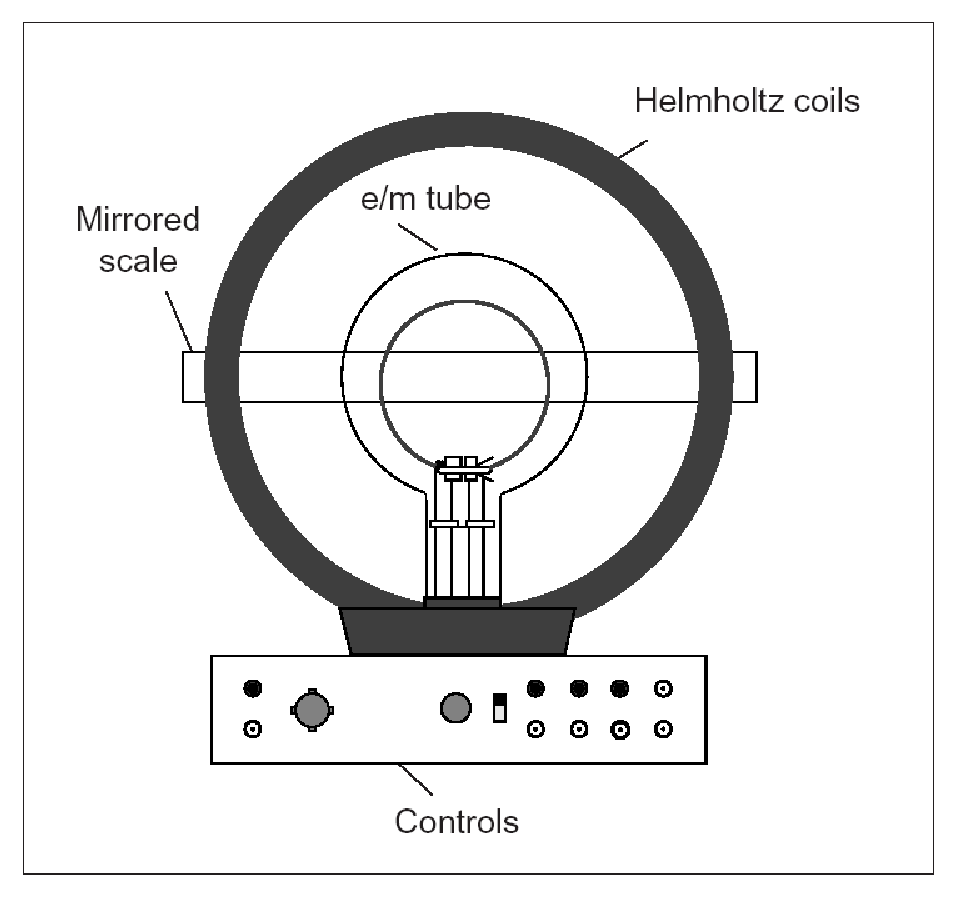
\includegraphics[height=3.5in]{eoverm/apparatus1.ps}

\caption{The $e/m$ apparatus.}

\end{center}
\end{figure}
The magnitude of the magnetic field along the axis of the pair of coils is
\begin{equation}
B = \left ( \frac{4}{5} \right )^{3/2} \frac{N \mu_0 I}{a}
\end{equation}
where $N$ is the number of turns of wire in each coil, $\mu_0$
is the permeability constant,  $I$ is the current in the coils,
and $a$ is the radius of the coil.
The direction of the field is parallel or anti-parallel
to the axis of the pair of coils depending on the direction of the current
in the coils.
The direction of the current is the same in each coil.
The magnetic field in the region between the coils is approximately equal
to the field along the axis of the coils so we will use
the expression above for our magnetic field in the equation you generated in
Activity 2.f.

\newpage

(a) Measure the radius of each coil of wire of the Helmholtz coils, 
average your results, and record them
below.
The number of turns of wire in each coil is $N=130$.
\vspace{15mm}


(b) Identify each item on the front panel below
the Helmholtz coils using Figure 3 as a guide.
Check that all the connections are correct using Figure 3 as your guide. 
\begin{figure}[hbt]
\begin{center}

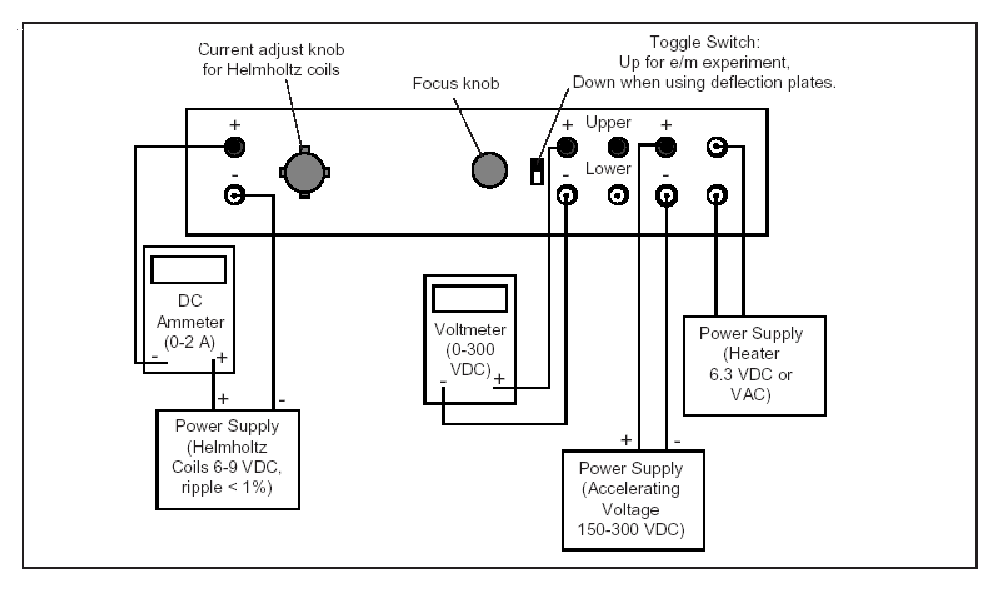
\includegraphics[height=3.5in]{eoverm/apparatus2.ps}

\caption{Instrument connections for the e/m experiment.}

\end{center}
\end{figure}

(c) Place the hood over the $e/m$ apparatus and flip the 
toggle switch up to the $e/m$ MEASURE
position.
Turn the current adjust knob for the Helmholtz coils to the vertical position (white line
at the 12 o'clock noon position).

(d) Identify the ammeter used to measure the current in the Helmholtz
coils using Figure 3 as a guide. 
Next, turn on the low-voltage power supply for the Helmholtz coils.
Now watch the current in the ammeter (it should not exceed $2~A$ under
any circumstances) and
turn up the voltage on the Helmholtz coils into the range of $6-9~V$.

(e) As you watch the ammeter slowly turn the current adjust knob for the Helmholtz
coils clockwise. Take care that
the current in the ammeter does not exceed $2 ~A$.
Set the current adjust knob for the Helmholtz coils in the $1.5-2.0~A$ range.

(f) Identify the power supply that runs the heater for the electron gun using Figure 3 as a guide
and turn on the power supply. Turn the voltage up to 6 volts.
{\bf CAUTION:} Do not exceed 6 volts or you may destroy the $e/m$
tube.

(g) Turn on the power supply for the accelerating voltage for the electron gun.
Turn the voltage up so that it is in the range of $150-300~V$.

(h) Wait several minutes for the cathode to heat up. When
it does, you will see the electron beam emerge from
the electron gun and it will be curved by the field from
the Helmholtz coils. If the electron beam is not sharp, adjust the focus knob. Check that the electron beam is parallel to the Helmholtz coils. If it is not, consult your instructor.
 Carefully read the current in the Helmholtz coils from
your ammeter and the accelerating voltage from your
voltmeter. Record the values below.
\vspace{25mm}

(i) Carefully measure the radius of the electron beam.
Look through the tube at the electron beam. To avoid
parallax errors, move your head to align the electron
beam with the reflection of the beam that you can see
on the mirrored scale. Measure the radius of the beam as you
see it on both sides of the scale, then average the results.
Record your results below.
\vspace{25mm}

(j) Slowly turn the current adjust knob for the Helmholtz
coils either up or down as you watch the ammeter and take care that
the current does not exceed $2 ~A$.
What parameter does this action effect, the magnetic field or the
accelerating voltage?
What happens to the path of the electrons as the current in the Helmholtz
coils changes?
Set the current adjust knob to some value and
repeat parts 4.h-i to get a second measurement. Record the current in the
Helmholtz coils, the accelerating voltage, and the average radius of the electron beam.
\vspace{30mm}

(k) Slowly change the accelerating voltage either up or down.
What parameter does this voltage effect? Consider your result for part 2.f.
What happens to the electron's path?
Set the accelerating voltage 
to some value and
repeat parts 4.h-i to get a third measurement. Record the current in the
Helmholtz coils, the accelerating voltage, and the average radius of the electron beam.
\vspace{30mm}

(l) When you are finished, turn down to zero the accelerating voltage, the heater voltage, the Helmholtz coil voltage, and the current adjust knob.
\vspace{10mm}

\newpage

\textbf{Activity 5: Extracting the Electron Mass From Your Data.}

(a) You should now have three separate measurements of the radius of the electron's path.
Use Equation 2 to calculate the magnitude of the magnetic field $B$
for each measurement.
\vspace{30mm}

(b) Almost there! Now calculate the electron mass for each of your three measurements using
the values of the average $r$, $V$, and $B$. 
Record your results below.
\vspace{50mm}

(c) Can you spot any trends in your results for the electron mass?
Try averaging the three results and determine the standard deviation.
Is your average and uncertainty consistent with the accepted value of the electron mass?
Is this averaging of your results acceptable in this situation?
Why?
What are the possible sources of uncertainty in this experiment?


%\begin{table}[h!]
%\begin{center}
%\begin{tabular}{|l|c|l|c|l|c|} \hline
%\hi Particle         & mass ($MeV/c^2$)  & Particle             & mass ($MeV/c^2$)  & Particle             & mass ($MeV/c^2$) \\ \hline
%\hi electron($e^-$)  & 0.511             & u-quark($u$)         & 1.5-4.0           & $\rm ^{12}C$         & 11,178 \\[2pt] \hline
%\hi positron($e^+$)  & 0.511             & neutrino($\nu_\tau$) & < 18.2            & $\rm ^{16}O$         & 14,904 \\[2pt] \hline
%\hi proton           & 938.27            & neutrino($\nu_e$)    & < 0.000003        & muon($\mu^+$)        & 105.66 \\[2pt] \hline
%\hi neutron          & 939.57            & neutrino($\nu_\mu$)  & < 0.19            & pion($\pi^+$)        & 139.57 \\[2pt] \hline
%\hi muon($\mu^-$)    & 105.66            & tau($\tau^-$)        & 1,777.0           & pion($\pi^-$)        & 139.57 \\[2pt] \hline
%\end{tabular}
%\caption{Some  particle masses.}
%\end{center}
%\end{table}

%\begin{table}[h!]
%\begin{center}
%\begin{tabular}{|l|c|l|c|} \hline
%\hi Particle         & mass ($MeV/c^2$)  & Particle             & mass ($MeV/c^2$) \\ \hline
%\hi electron($e^-$)  & 0.511             & $\rm ^{12}C$         & 11,178 \\[2pt] \hline
%\hi positron($e^+$)  & 0.511             & $\rm ^{16}O$         & 14,904 \\[2pt] \hline
%\hi proton           & 938.27            & muon($\mu^+$)        & 105.66 \\[2pt] \hline
%\hi neutron          & 939.57            & pion($\pi^+$)        & 139.57 \\[2pt] \hline
%\hi muon($\mu^-$)    & 105.66            & tau($\tau^-$)        & 1,777.0 \\[2pt] \hline
%\hi neutrino($\nu_e$)& < 0.000003        & neutrino($\nu_\mu$)  & < 0.19 \\[2pt] \hline
%\hi u-quark($u$)     & 1.5-4.0           & neutrino($\nu_\tau$) & < 18.2 \\[2pt] \hline
%\end{tabular}
%\caption{Some atomic and sub-atomic particle masses.}
%\end{center}
%\end{table}

